\chapter{Testing}
At first time running the algorithm, the input vision for the ball to the wave was from the centre of the ball to both sides of the wave as a single point. That made it hard for the ball to find its way (or have a futuristic vision, as you can say). There would be a change in the wave curve and the ball couldn't detect it, so the idea came of having more range for the ball to see. It would calculate the distance between the ball rectangle and the left or right side of the wave in more than one point.

To get more into it with numbers, there would be a notice of the ball having a weird sense of getting to know its "new" sense of wider vision diameter. The ball would take about 20 generations just to start moving more randomly left and right. This is made when the ball had only the vision of its 24-pixel diameter (12 px as radius) and then the extra step of plus 50 pixels, getting this info in a nutshell.
\begin{itemize}
	\item One point vision: good as start and better CPU wise.
	\item Diameter vision + 20: best one in score yet (117 points in generation 89).
	\item Diameter +50 points: No learning even after nearly 300 generation.
\end{itemize}

The reason to increase the vision for the ball (even though it was working fine) is that I wanted to test how long it would take for the ball to get used to the new (increased) amount of lines. I can tell you that it took long enough.

\begin{figure}[H]
	\centering
	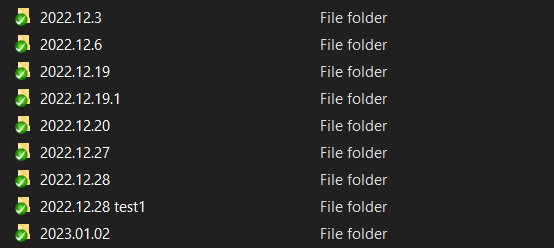
\includegraphics[width=0.7\linewidth]{usedImages/numTrainingSessions}
	\caption[]{Number of training sessions}
	\label{fig:numtrainingsessions}
\end{figure}


At this point in the game, I implemented the increased speed of wave *4 that improved the learning speed. With normal fps, it would take 8 hours and 15 minutes for 37 generations, but the new one (with a limitation of 4 times the speed, not more) takes 5 hours and 15 minutes for 100 generations to work. That is four times the normal running time of a normal pace of game for a human to play it, and the generation threshold to be 300 generation instead of 100. Let the laptop run as much as it needs. It took more than 15 hours to finish 294 generations and 11 genomes, when I went back to check the log, none of them managed to pass the 3000 fitness score. That means that none of them had a good intuition about the lines to move left or right and at least overcome one curve in the wave. From this, the amount of numbers increased = more time in training.

There is a small box that is shown around the ball, it is called ballRect and is mentioned a lot in the \hyperref[sec:count-distance]{Count Distance} and \hyperref[sec:collision]{Collision}. ballRect is shown to check if the genome did terminate for an actual collision or because it reached the threshold, like the case here in this video.

In order to save as much CPU power as possible during the learning process, the box is shown only when fitness is over 50. In addition to some extra visuals in the game, such as the particles behind the ball, all of them can be viewed again with a key for each one:
\begin{itemize}
	\item \inlineCode{v Key} to shown \textbf{v}ision
	\item \inlineCode{b key} to show the \textbf{b}allRect
	\item \inlineCode{p key} to show the \textbf{p}articles
\end{itemize}